% Created by tikzDevice version 0.12.3.1 on 2022-09-02 13:46:34
% !TEX encoding = UTF-8 Unicode
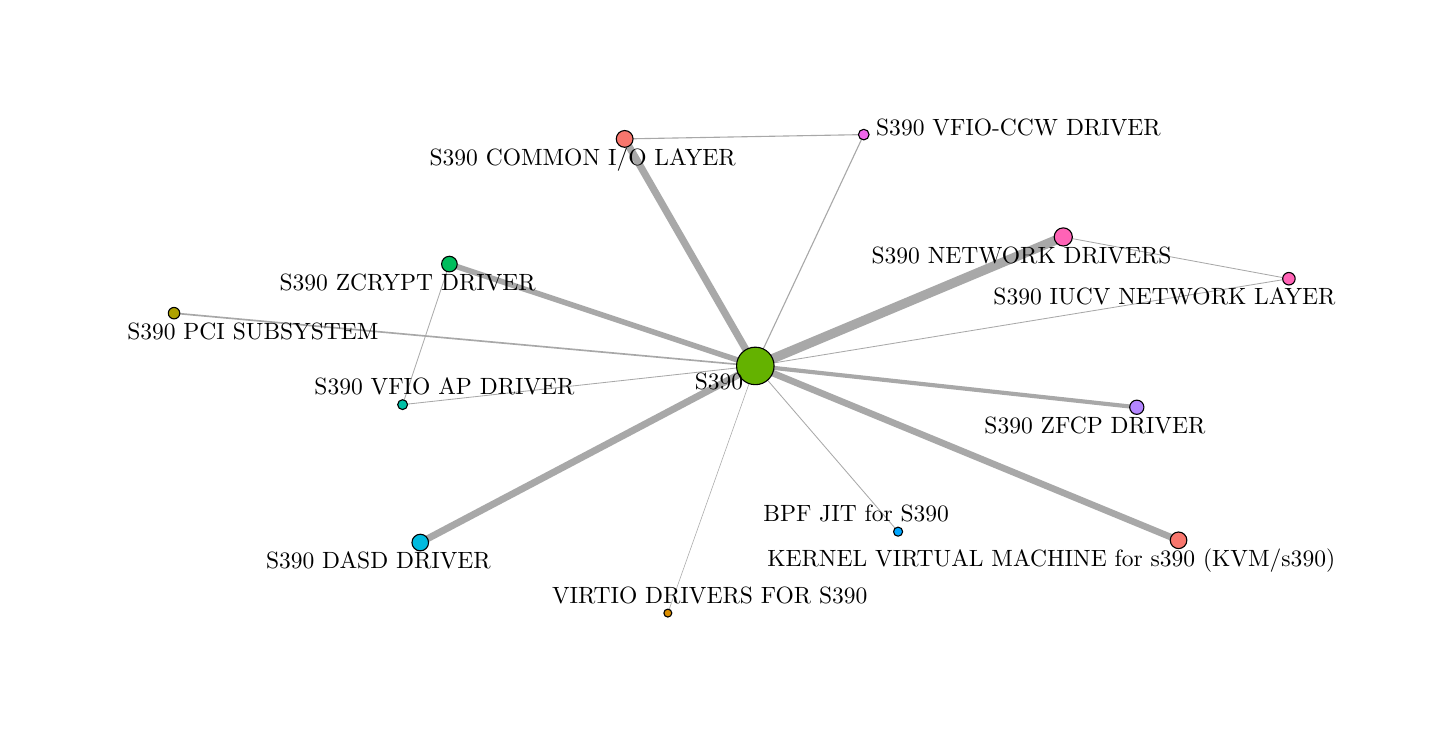
\begin{tikzpicture}[x=1pt,y=1pt]
\definecolor{fillColor}{RGB}{255,255,255}
\path[use as bounding box,fill=fillColor,fill opacity=0.00] (0,0) rectangle (505.89,252.94);
\begin{scope}
\path[clip] (  0.00,  0.00) rectangle (505.89,252.94);
\definecolor{fillColor}{RGB}{255,255,255}

\path[fill=fillColor] (  0.00,  0.00) rectangle (505.89,252.94);
\end{scope}
\begin{scope}
\path[clip] ( 32.75, 32.75) rectangle (475.89,222.94);
\definecolor{drawColor}{gray}{0.66}

\path[draw=drawColor,line width= 0.3pt,line join=round] (314.52, 70.82) -- (262.93,130.71);

\path[draw=drawColor,line width= 2.4pt,line join=round] (415.87, 67.70) -- (262.93,130.71);

\path[draw=drawColor,line width= 2.6pt,line join=round] (262.93,130.71) -- (215.72,212.74);

\path[draw=drawColor,line width= 2.5pt,line join=round] (262.93,130.71) -- (141.86, 66.89);

\path[draw=drawColor,line width= 0.3pt,line join=round] (262.93,130.71) -- (455.75,162.22);

\path[draw=drawColor,line width= 3.4pt,line join=round] (262.93,130.71) -- (374.21,177.32);

\path[draw=drawColor,line width= 0.6pt,line join=round] (262.93,130.71) -- ( 52.89,149.77);

\path[draw=drawColor,line width= 0.3pt,line join=round] (262.93,130.71) -- (135.48,116.72);

\path[draw=drawColor,line width= 0.4pt,line join=round] (262.93,130.71) -- (302.12,214.30);

\path[draw=drawColor,line width= 2.0pt,line join=round] (262.93,130.71) -- (152.39,167.51);

\path[draw=drawColor,line width= 1.5pt,line join=round] (262.93,130.71) -- (400.78,115.78);

\path[draw=drawColor,line width= 0.2pt,line join=round] (262.93,130.71) -- (231.32, 41.40);

\path[draw=drawColor,line width= 0.4pt,line join=round] (215.72,212.74) -- (302.12,214.30);

\path[draw=drawColor,line width= 0.3pt,line join=round] (455.75,162.22) -- (374.21,177.32);

\path[draw=drawColor,line width= 0.3pt,line join=round] (135.48,116.72) -- (152.39,167.51);
\definecolor{drawColor}{RGB}{0,0,0}
\definecolor{fillColor}{RGB}{0,166,255}

\path[draw=drawColor,line width= 0.4pt,line join=round,line cap=round,fill=fillColor] (314.52, 70.82) circle (  1.65);
\definecolor{fillColor}{RGB}{248,118,109}

\path[draw=drawColor,line width= 0.4pt,line join=round,line cap=round,fill=fillColor] (415.87, 67.70) circle (  3.00);
\definecolor{fillColor}{RGB}{100,178,0}

\path[draw=drawColor,line width= 0.4pt,line join=round,line cap=round,fill=fillColor] (262.93,130.71) circle (  6.78);
\definecolor{fillColor}{RGB}{248,118,109}

\path[draw=drawColor,line width= 0.4pt,line join=round,line cap=round,fill=fillColor] (215.72,212.74) circle (  3.03);
\definecolor{fillColor}{RGB}{0,186,222}

\path[draw=drawColor,line width= 0.4pt,line join=round,line cap=round,fill=fillColor] (141.86, 66.89) circle (  3.00);
\definecolor{fillColor}{RGB}{255,99,182}

\path[draw=drawColor,line width= 0.4pt,line join=round,line cap=round,fill=fillColor] (455.75,162.22) circle (  2.26);

\path[draw=drawColor,line width= 0.4pt,line join=round,line cap=round,fill=fillColor] (374.21,177.32) circle (  3.28);
\definecolor{fillColor}{RGB}{174,162,0}

\path[draw=drawColor,line width= 0.4pt,line join=round,line cap=round,fill=fillColor] ( 52.89,149.77) circle (  2.07);
\definecolor{fillColor}{RGB}{0,193,167}

\path[draw=drawColor,line width= 0.4pt,line join=round,line cap=round,fill=fillColor] (135.48,116.72) circle (  1.78);
\definecolor{fillColor}{RGB}{239,103,235}

\path[draw=drawColor,line width= 0.4pt,line join=round,line cap=round,fill=fillColor] (302.12,214.30) circle (  1.92);
\definecolor{fillColor}{RGB}{0,189,92}

\path[draw=drawColor,line width= 0.4pt,line join=round,line cap=round,fill=fillColor] (152.39,167.51) circle (  2.82);
\definecolor{fillColor}{RGB}{179,133,255}

\path[draw=drawColor,line width= 0.4pt,line join=round,line cap=round,fill=fillColor] (400.78,115.78) circle (  2.57);
\definecolor{fillColor}{RGB}{219,142,0}

\path[draw=drawColor,line width= 0.4pt,line join=round,line cap=round,fill=fillColor] (231.32, 41.40) circle (  1.43);

\node[text=drawColor,anchor=base,inner sep=0pt, outer sep=0pt, scale=  0.85] at (299.38, 74.38) {BPF JIT for S390};

\node[text=drawColor,anchor=base,inner sep=0pt, outer sep=0pt, scale=  0.85] at (369.88, 58.29) {KERNEL VIRTUAL MACHINE for s390 (KVM/s390)};

\node[text=drawColor,anchor=base,inner sep=0pt, outer sep=0pt, scale=  0.85] at (249.81,122.14) {S390};

\node[text=drawColor,anchor=base,inner sep=0pt, outer sep=0pt, scale=  0.85] at (200.55,203.29) {S390 COMMON I/O LAYER};

\node[text=drawColor,anchor=base,inner sep=0pt, outer sep=0pt, scale=  0.85] at (126.74, 57.46) {S390 DASD DRIVER};

\node[text=drawColor,anchor=base,inner sep=0pt, outer sep=0pt, scale=  0.85] at (410.80,152.80) {S390 IUCV NETWORK LAYER};

\node[text=drawColor,anchor=base,inner sep=0pt, outer sep=0pt, scale=  0.85] at (359.13,167.90) {S390 NETWORK DRIVERS};

\node[text=drawColor,anchor=base,inner sep=0pt, outer sep=0pt, scale=  0.85] at ( 81.38,140.33) {S390 PCI SUBSYSTEM};

\node[text=drawColor,anchor=base,inner sep=0pt, outer sep=0pt, scale=  0.85] at (150.62,120.28) {S390 VFIO AP DRIVER};

\node[text=drawColor,anchor=base,inner sep=0pt, outer sep=0pt, scale=  0.85] at (358.02,214.05) {S390 VFIO-CCW DRIVER};

\node[text=drawColor,anchor=base,inner sep=0pt, outer sep=0pt, scale=  0.85] at (137.33,158.09) {S390 ZCRYPT DRIVER};

\node[text=drawColor,anchor=base,inner sep=0pt, outer sep=0pt, scale=  0.85] at (385.65,106.36) {S390 ZFCP DRIVER};

\node[text=drawColor,anchor=base,inner sep=0pt, outer sep=0pt, scale=  0.85] at (246.46, 44.96) {VIRTIO DRIVERS FOR S390};
\end{scope}
\end{tikzpicture}
